% ─── Chapter 4: Full Order Model ─────────────────────────────────────────────

% Slide: Governing Dynamic Equations (from thesis Ch.4)
\begin{frame}{Governing Dynamic Equations}
  \small
  To simulate the dynamic response we resolve the semi-discrete system:
  \begin{block}{Equation of Motion}
    \vspace{-0.15cm}
    \[
      \mat{M}(\boldsymbol{\mu})\,\ddot{\vect{U}}(t) + \mat{C}(\boldsymbol{\mu})\,\dot{\vect{U}}(t) + \mat{K}(\boldsymbol{\mu})\,\vect{U}(t) = \lambda(t)\,\vect{F}_{\text{ext}}
    \]
    \vspace{-0.45cm}
    \[
      \text{with initial conditions: } \vect{U}(0) = \vect{U}_0, \quad \dot{\vect{U}}(0) = \vect{V}_0
    \]
    \vspace{-0.15cm}
  \end{block}
  \begin{columns}[T]
    \begin{column}{0.52\textwidth}
      \textbf{Element mass matrix}:
      \[
        \mat{M}_{e,ab} = \int_{-1}^1\!\int_{-1}^1 \rho\,R_a R_b\,|J(\xi,\eta)|\,d\xi\,d\eta
      \]
      \vspace{-0.1cm}
      \textbf{Rayleigh damping}: $\mat{C}(\boldsymbol{\mu}) = \alpha_M\mat{M}(\boldsymbol{\mu}) + \beta_K\mat{K}(\boldsymbol{\mu})$
    \end{column}
    \begin{column}{0.45\textwidth}
      \textbf{Element stiffness matrix}:
      \[
        \mat{K}_{e,ab}(\boldsymbol{\mu}) = \int_{-1}^{1}\!\int_{-1}^{1}\mat{B}_a^T\mat{D}\mat{B}_b\,|J(\xi,\eta;\boldsymbol{\mu})|\,d\xi\,d\eta
      \]
      \vspace{-0.1cm}
      \begin{alertblock}{Online Assembly Bottleneck}
        \footnotesize
        As $\boldsymbol{\mu}$ changes, $\mat{J}(\xi,\eta;\boldsymbol{\mu})$ varies at every Gauss point $\Rightarrow$ full mesh re-assembly is required at each time step.
      \end{alertblock}
    \end{column}
  \end{columns}
\end{frame}

% Slide: Simulation Path & Solver Workflow
\begin{frame}{Simulation Path \& Solver Workflow}
  \centering
  \scalebox{1}{
    \begin{tikzpicture}[
        node distance=1.4cm,
        row1/.style={rectangle, draw=blue!70, fill=blue!5, thick, rounded corners, minimum width=5.8cm, minimum height=0.7cm, align=center, font=\sffamily\scriptsize},
        row2/.style={rectangle, draw=teal!70, fill=teal!5, thick, rounded corners, minimum width=5.8cm, minimum height=0.7cm, align=center, font=\sffamily\scriptsize},
        row3/.style={rectangle, draw=orange!70, fill=orange!5, thick, rounded corners, minimum width=5.8cm, minimum height=0.7cm, align=center, font=\sffamily\scriptsize},
        row4/.style={rectangle, draw=purple!70, fill=purple!5, thick, rounded corners, minimum width=5.8cm, minimum height=0.7cm, align=center, font=\sffamily\scriptsize},
        row5/.style={rectangle, draw=olive!70, fill=olive!5, thick, rounded corners, minimum width=5.8cm, minimum height=0.7cm, align=center, font=\sffamily\scriptsize},
        arrow/.style={thick,->,>=stealth}
      ]
      % Left Column: Classical Physical-Domain
      \node [row1] (l1) {\textbf{Classical Physical Path} \\ Goal: $\int_{\Omega(\boldsymbol{\mu})} \dots \mathrm{d}\Omega$ (physical domain)};
      \node [row2, below of=l1] (l2) {Basis Functions \\ $R_i(\boldsymbol{\mu})$ varies (mesh regenerated)};
      \node [row3, below of=l2] (l3) {Online Assembly \\ Assemble $\mat{K}(\boldsymbol{\mu})$, $\mat{M}(\boldsymbol{\mu})$ (expensive)};
      \node [row4, below of=l3] (l4) {Implicit Time Scheme \\ Newmark-$\beta$ Solver};
      \node [row5, below of=l4] (l5) {Extract QoI \\ Tip deflection $U_y(t)$ \& $\sigma_{\text{VM}}$ (variable dimensions)};

      % Right Column: Mapped Reference
      \node [row1, right=1.6cm of l1] (r1) {\textbf{Reference Map Path} \\ Goal: $\int_{\hat{\Omega}} \dots J_{\boldsymbol{\mu}}\,\mathrm{d}\hat{\Omega}$ (fixed reference domain)};
      \node [row2, below of=r1] (r2) {Bases Remain the Same \\ $\hat{R}_i$ is parameter-independent};
      \node [row3, below of=r2] (r3) {Pulled-Back Assembly \\ $\hat{\mat{K}}(\boldsymbol{\mu}), \hat{\mat{M}}(\boldsymbol{\mu})$ depend on $J(\boldsymbol{\mu})$ (online) \\ Shape derivatives pre-computed};
      \node [row4, below of=r3] (r4) {Implicit Time Scheme \\ Newmark-$\beta$ Solver \\ \textcolor{red!80!black}{\scriptsize(possibility of ill-conditioning)}};
      \node [row5, below of=r4] (r5) {Extract QoI \\ Tip deflection $U_y(t)$ \& $\sigma_{\text{VM}}$ (constant dimensions)};

      % ROM Application Labels (Outside Flowchart, on the Right)
      \node [red!80!black, font=\sffamily\tiny\bfseries, align=center, right=0.15cm of r3] (rom3_label) {$\gets$ Hyper-Reduction\\(reduces elements: $N_e \to M_e$)};
      \node [red!80!black, font=\sffamily\tiny\bfseries, align=center, right=0.15cm of r4] (rom4_label) {$\gets$ Galerkin ROM\\(reduces DOFs: $N \to r$)};

      % Connections
      \draw [arrow] (l1) -- (l2);
      \draw [arrow] (l2) -- (l3);
      \draw [arrow] (l3) -- (l4);
      \draw [arrow] (l4) -- (l5);

      \draw [arrow] (r1) -- (r2);
      \draw [arrow] (r2) -- (r3);
      \draw [arrow] (r3) -- (r4);
      \draw [arrow] (r4) -- (r5);
    \end{tikzpicture}
  }
\end{frame}

% Slide: Model Displacement Field
\begin{frame}{Model Displacement Field}
  \begin{columns}[T]
    \begin{column}{0.45\textwidth}
      \small
      \textbf{Deflection Contours}:
      \begin{itemize}
        \item Represents the physical displacement magnitude across the 2D surface.
        \item Transitions smoothly from \textbf{zero} at the clamped boundary ($x=0$) to a \textbf{maximum} at the loaded free tip ($x=L$).
        \item \textbf{Quantity of Interest (QoI)}: Tip vertical deflection $U_y(t)$ is measured at the free edge.
      \end{itemize}
    \end{column}
    \begin{column}{0.52\textwidth}
      \centering
      \scalebox{0.65}{
        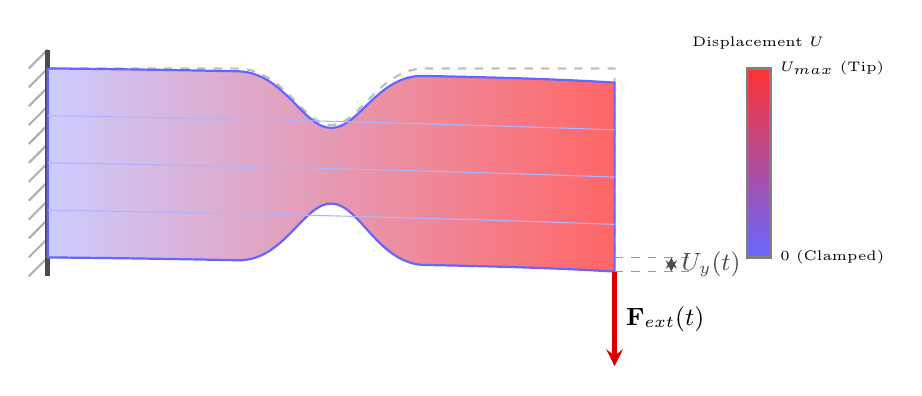
\begin{tikzpicture}[scale=1.2, >=stealth]
          % --- UNDEFORMED REFERENCE STATE (dashed) ---
          \draw[dashed, black!25, thick]
          (0, 1.0) -- (2.0, 1.0)
          .. controls (2.5, 1.0) and (2.7, 0.4) .. (3.0, 0.4)
          .. controls (3.3, 0.4) and (3.5, 1.0) .. (4.0, 1.0)
          -- (6.0, 1.0) -- (6.0, -1.0) -- (4.0, -1.0)
          .. controls (3.5, -1.0) and (3.3, -0.4) .. (3.0, -0.4)
          .. controls (2.7, -0.4) and (2.5, -1.0) .. (2.0, -1.0)
          -- (0, -1.0) -- cycle;
          \node[black!40, font=\small] at (4.5, 0.3) {Undeformed};

          % --- CLAMPED BOUNDARY HATCHING ---
          \foreach \y in {-1.2, -1.0, -0.8, -0.6, -0.4, -0.2, 0.0, 0.2, 0.4, 0.6, 0.8, 1.0} {
              \draw[thick, black!30] (-0.2, \y) -- (0, \y+0.2);
            }
          \draw[ultra thick, black!70] (0, -1.2) -- (0, 1.2);

          % --- DEFORMED STRUCTURE WITH DISPLACEMENT CONTOUR ---
          \begin{scope}
            \clip (0, 1.0)
            .. controls (1.0, 0.99) and (1.5, 0.98) .. (2.0, 0.97)
            .. controls (2.5, 0.97) and (2.7, 0.37) .. (3.0, 0.37)
            .. controls (3.3, 0.37) and (3.5, 0.95) .. (4.0, 0.92)
            .. controls (5.0, 0.9) and (5.5, 0.88) .. (6.0, 0.85)
            -- (6.0, -1.15)
            .. controls (5.5, -1.12) and (5.0, -1.1) .. (4.0, -1.08)
            .. controls (3.5, -1.08) and (3.3, -0.43) .. (3.0, -0.43)
            .. controls (2.7, -0.43) and (2.5, -1.05) .. (2.0, -1.03)
            .. controls (1.5, -1.02) and (1.0, -1.01) .. (0, -1.0)
            -- cycle;

            % Horizontal gradient representing displacement increasing from left to right
            \path[shading=xgradient, left color=blue!20, right color=red!60] (0, -2.0) rectangle (6.0, 2.0);
          \end{scope}

          % Draw the boundary of the deformed notched plate
          \draw[draw=blue!60, thick] (0, 1.0)
          .. controls (1.0, 0.99) and (1.5, 0.98) .. (2.0, 0.97)
          .. controls (2.5, 0.97) and (2.7, 0.37) .. (3.0, 0.37)
          .. controls (3.3, 0.37) and (3.5, 0.95) .. (4.0, 0.92)
          .. controls (5.0, 0.9) and (5.5, 0.88) .. (6.0, 0.85)
          -- (6.0, -1.15)
          .. controls (5.5, -1.12) and (5.0, -1.1) .. (4.0, -1.08)
          .. controls (3.5, -1.08) and (3.3, -0.43) .. (3.0, -0.43)
          .. controls (2.7, -0.43) and (2.5, -1.05) .. (2.0, -1.03)
          .. controls (1.5, -1.02) and (1.0, -1.01) .. (0, -1.0)
          -- cycle;

          \draw[blue!30, thin] (0, 0) .. controls (2.0, -0.03) and (4.0, -0.08) .. (6.0, -0.15);
          \draw[blue!30, thin] (0, 0.5) .. controls (2.0, 0.47) and (4.0, 0.42) .. (6.0, 0.35);
          \draw[blue!30, thin] (0, -0.5) .. controls (2.0, -0.53) and (4.0, -0.58) .. (6.0, -0.65);

          % --- LOADING FORCE ARROW ---
          \draw[->, ultra thick, red!85!black] (6.0, -1.15) -- node[right, font=\small, black] {$\mathbf{F}_{\text{ext}}(t)$} (6.0, -2.15);

          % --- DEFLECTION INDICATORS ---
          \draw[dashed, black!40] (6.0, -1.0) -- (6.8, -1.0);
          \draw[dashed, black!40] (6.0, -1.15) -- (6.8, -1.15);
          \draw[<->, thick, black!70] (6.6, -1.0) -- node[right, font=\small] {$U_y(t)$} (6.6, -1.15);

          % --- COLORBAR ---
          \begin{scope}[xshift=7.4cm, yshift=-1.0cm]
            \path[shading=ygradient, top color=red!80, bottom color=blue!60] (0, 0) rectangle (0.25, 2.0);
            \draw[thick, black!50] (0, 0) rectangle (0.25, 2.0);
            \node[right, font=\tiny] at (0.25, 2.0) {$U_{\text{max}}$ (Tip)};
            \node[right, font=\tiny] at (0.25, 0.0) {$0$ (Clamped)};
            \node[above, font=\tiny, align=center] at (0.12, 2.1) {Displacement $U$};
          \end{scope}
        \end{tikzpicture}
      }
    \end{column}
  \end{columns}
\end{frame}

% Slide: Model Stress & Von Mises Definition
\begin{frame}{Model Stress \& Von Mises Definition}
  \begin{columns}[T]
    \begin{column}{0.45\textwidth}
      \small
      \textbf{Stress Reconstruction}:
      \begin{itemize}
        \item \textbf{Key Relation}: Once the displacement field $\vect{u}$ is solved, we evaluate strain $\boldsymbol{\varepsilon}(\vect{u})$, constitutive stress $\boldsymbol{\sigma} = \mat{D}:\boldsymbol{\varepsilon}$, and reconstructed yield criteria.
        \item \textbf{Von Mises Stress $\sigma_{\text{VM}}$}:
              \[
                \sigma_{\text{VM}} = \sqrt{ \sigma_{xx}^2 - \sigma_{xx}\sigma_{yy} + \sigma_{yy}^2 + 3\tau_{xy}^2 }
              \]
        \item \textbf{Stress Concentration}: Localized at notch throats (mechanical fatigue risk).
      \end{itemize}
    \end{column}
    \begin{column}{0.52\textwidth}
      \centering
      \scalebox{0.65}{
        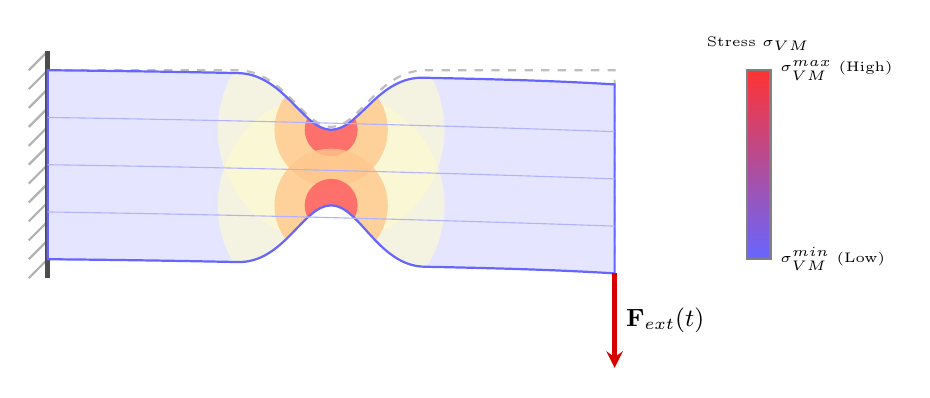
\begin{tikzpicture}[scale=1.2, >=stealth]
          % --- UNDEFORMED REFERENCE STATE (dashed) ---
          \draw[dashed, black!25, thick]
          (0, 1.0) -- (2.0, 1.0)
          .. controls (2.5, 1.0) and (2.7, 0.4) .. (3.0, 0.4)
          .. controls (3.3, 0.4) and (3.5, 1.0) .. (4.0, 1.0)
          -- (6.0, 1.0) -- (6.0, -1.0) -- (4.0, -1.0)
          .. controls (3.5, -1.0) and (3.3, -0.4) .. (3.0, -0.4)
          .. controls (2.7, -0.4) and (2.5, -1.0) .. (2.0, -1.0)
          -- (0, -1.0) -- cycle;
          \node[black!40, font=\small] at (4.5, 0.3) {Undeformed};

          % --- CLAMPED BOUNDARY HATCHING ---
          \foreach \y in {-1.2, -1.0, -0.8, -0.6, -0.4, -0.2, 0.0, 0.2, 0.4, 0.6, 0.8, 1.0} {
              \draw[thick, black!30] (-0.2, \y) -- (0, \y+0.2);
            }
          \draw[ultra thick, black!70] (0, -1.2) -- (0, 1.2);

          % --- DEFORMED STRUCTURE WITH STRESS CONCENTRATION ---
          \begin{scope}
            \clip (0, 1.0)
            .. controls (1.0, 0.99) and (1.5, 0.98) .. (2.0, 0.97)
            .. controls (2.5, 0.97) and (2.7, 0.37) .. (3.0, 0.37)
            .. controls (3.3, 0.37) and (3.5, 0.95) .. (4.0, 0.92)
            .. controls (5.0, 0.9) and (5.5, 0.88) .. (6.0, 0.85)
            -- (6.0, -1.15)
            .. controls (5.5, -1.12) and (5.0, -1.1) .. (4.0, -1.08)
            .. controls (3.5, -1.08) and (3.3, -0.43) .. (3.0, -0.43)
            .. controls (2.7, -0.43) and (2.5, -1.05) .. (2.0, -1.03)
            .. controls (1.5, -1.02) and (1.0, -1.01) .. (0, -1.0)
            -- cycle;

            \fill[blue!10] (-0.5, -3.0) rectangle (7.0, 2.0);
            \draw[fill=yellow!20, draw=none, opacity=0.6] (3.0, 0.37) circle (1.2);
            \draw[fill=yellow!20, draw=none, opacity=0.6] (3.0, -0.43) circle (1.2);
            \draw[fill=orange!45, draw=none, opacity=0.8] (3.0, 0.37) circle (0.6);
            \draw[fill=red!60, draw=none, opacity=0.9] (3.0, 0.37) circle (0.28);
            \draw[fill=orange!45, draw=none, opacity=0.8] (3.0, -0.43) circle (0.6);
            \draw[fill=red!60, draw=none, opacity=0.9] (3.0, -0.43) circle (0.28);
          \end{scope}

          % Draw the boundary of the deformed notched plate
          \draw[draw=blue!60, thick] (0, 1.0)
          .. controls (1.0, 0.99) and (1.5, 0.98) .. (2.0, 0.97)
          .. controls (2.5, 0.97) and (2.7, 0.37) .. (3.0, 0.37)
          .. controls (3.3, 0.37) and (3.5, 0.95) .. (4.0, 0.92)
          .. controls (5.0, 0.9) and (5.5, 0.88) .. (6.0, 0.85)
          -- (6.0, -1.15)
          .. controls (5.5, -1.12) and (5.0, -1.1) .. (4.0, -1.08)
          .. controls (3.5, -1.08) and (3.3, -0.43) .. (3.0, -0.43)
          .. controls (2.7, -0.43) and (2.5, -1.05) .. (2.0, -1.03)
          .. controls (1.5, -1.02) and (1.0, -1.01) .. (0, -1.0)
          -- cycle;

          \draw[blue!30, thin] (0, 0) .. controls (2.0, -0.03) and (4.0, -0.08) .. (6.0, -0.15);
          \draw[blue!30, thin] (0, 0.5) .. controls (2.0, 0.47) and (4.0, 0.42) .. (6.0, 0.35);
          \draw[blue!30, thin] (0, -0.5) .. controls (2.0, -0.53) and (4.0, -0.58) .. (6.0, -0.65);

          % --- LOADING FORCE ARROW ---
          \draw[->, ultra thick, red!85!black] (6.0, -1.15) -- node[right, font=\small, black] {$\mathbf{F}_{\text{ext}}(t)$} (6.0, -2.15);

          % --- COLORBAR ---
          \begin{scope}[xshift=7.4cm, yshift=-1.0cm]
            \path[shading=ygradient, top color=red!80, bottom color=blue!60] (0, 0) rectangle (0.25, 2.0);
            \draw[thick, black!50] (0, 0) rectangle (0.25, 2.0);
            \node[right, font=\tiny] at (0.25, 2.0) {$\sigma_{\text{VM}}^{\text{max}}$ (High)};
            \node[right, font=\tiny] at (0.25, 0.0) {$\sigma_{\text{VM}}^{\text{min}}$ (Low)};
            \node[above, font=\tiny, align=center] at (0.12, 2.1) {Stress $\sigma_{\text{VM}}$};
          \end{scope}
        \end{tikzpicture}
      }
    \end{column}
  \end{columns}
\end{frame}

% Slide: Full Order Model: Validation
\begin{frame}{Physical vs. Reference Mapped Path: Validation}
  \begin{columns}[T]
    \begin{column}{0.48\textwidth}
      \small
      \textbf{Numerical Validation}:
      \begin{itemize}
        \item Compare the transient vertical deflection $U_y(t)$ computed via both pathways.
        \item \textbf{Exact Agreement}: Near-zero difference validates the mathematical consistency of the pullback transformation.
      \end{itemize}
    \end{column}
    \begin{column}{0.48\textwidth}
      \centering
      \scalebox{0.72}{
        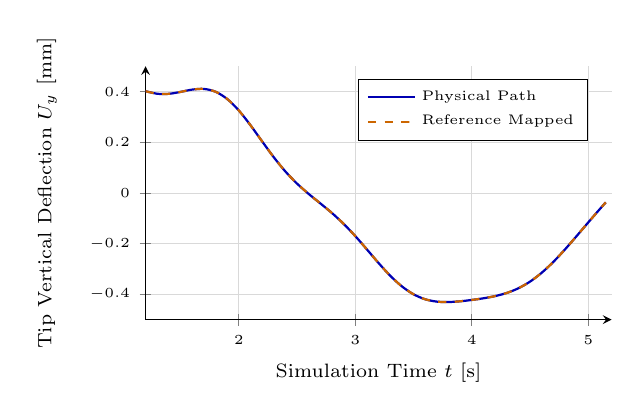
\begin{tikzpicture}
          \begin{axis}[
              width=7.5cm,
              height=4.8cm,
              xlabel={Simulation Time $t$ [s]},
              ylabel={Tip Vertical Deflection $U_y$ [mm]},
              xmin=1.2, xmax=5.2,
              ymin=-0.5, ymax=0.5,
              grid=both,
              grid style={line width=.1pt, draw=gray!15},
              major grid style={line width=.2pt, draw=gray!30},
              axis lines=left,
              enlargelimits=false,
              tick label style={font=\tiny},
              xlabel style={font=\scriptsize},
              ylabel style={font=\scriptsize, yshift=0.5em},
              legend style={at={(0.95,0.95)}, anchor=north east, font=\tiny, cells={anchor=west}},
            ]
            \addplot[
              color=blue!70!black,
              thick,
              smooth,
              mark=none
            ] coordinates {
                (1.2, 0.4014) (1.3, 0.3913) (1.4, 0.3910) (1.5, 0.3986)
                (1.6, 0.4077) (1.7, 0.4104) (1.8, 0.3994) (1.9, 0.3710)
                (2.0, 0.3256) (2.1, 0.2675) (2.2, 0.2037) (2.3, 0.1410)
                (2.4, 0.0847) (2.5, 0.0368) (2.6, -0.0040) (2.7, -0.0413)
                (2.8, -0.0794) (2.9, -0.1220) (3.0, -0.1703) (3.1, -0.2230)
                (3.2, -0.2767) (3.3, -0.3268) (3.4, -0.3688) (3.5, -0.4000)
                (3.6, -0.4197) (3.7, -0.4290) (3.8, -0.4306) (3.9, -0.4277)
                (4.0, -0.4224) (4.1, -0.4158) (4.2, -0.4072) (4.3, -0.3948)
                (4.4, -0.3764) (4.5, -0.3501) (4.6, -0.3152) (4.7, -0.2723)
                (4.8, -0.2231) (4.9, -0.1703) (5.0, -0.1163) (5.1, -0.0633)
                (5.15, -0.0375)
              };
            \addlegendentry{Physical Path}

            \addplot[
              color=orange!80!black,
              thick,
              dashed,
              smooth,
              mark=none
            ] coordinates {
                (1.2, 0.4014) (1.3, 0.3913) (1.4, 0.3910) (1.5, 0.3986)
                (1.6, 0.4077) (1.7, 0.4104) (1.8, 0.3994) (1.9, 0.3710)
                (2.0, 0.3256) (2.1, 0.2675) (2.2, 0.2037) (2.3, 0.1410)
                (2.4, 0.0847) (2.5, 0.0368) (2.6, -0.0040) (2.7, -0.0413)
                (2.8, -0.0794) (2.9, -0.1220) (3.0, -0.1703) (3.1, -0.2230)
                (3.2, -0.2767) (3.3, -0.3268) (3.4, -0.3688) (3.5, -0.4000)
                (3.6, -0.4197) (3.7, -0.4290) (3.8, -0.4306) (3.9, -0.4277)
                (4.0, -0.4224) (4.1, -0.4158) (4.2, -0.4072) (4.3, -0.3948)
                (4.4, -0.3764) (4.5, -0.3501) (4.6, -0.3152) (4.7, -0.2723)
                (4.8, -0.2231) (4.9, -0.1703) (5.0, -0.1163) (5.1, -0.0633)
                (5.15, -0.0375)
              };
            \addlegendentry{Reference Mapped}
          \end{axis}
        \end{tikzpicture}
      }
      \\[2pt]
      {\scriptsize Tip vertical deflection $U_y(t)$ transient curve}
    \end{column}
  \end{columns}
\end{frame}
